%! TeX program = xelatex
\newcommand{\PFF}[1]{./body/aux/learning/#1}
\documentclass[../ml-ct.tex]{subfiles}
\begin{document}
\chapter{Towards Learning a True Prior}%
\label{chap:reconstruction}
\myepigraph{All models are wrong, but some are useful.}{George E. P. Box}{Robustness in the Strategy of Scientific Model Building}

\minitoc%
In the previous chapters, we discussed the physical principles of \gls{ct}, went over the image formation, and glimpsed at the differences and advantages or drawbacks of solving the continuous and discretized models.
In this chapter, we will focus on reconstruction in the discretized model.
Specifically, we will first discuss different strategies for guiding the reconstruction towards plausible solutions given the measurement uncertainties and resulting artifacts that were discussed previously.
Then, we will shift our focus towards developing the theory behind the specific approach that we follow throughout this thesis.

Recall that, in essence, we aim to (in some sense) solve the linear system
\begin{equation}
	p = Af + \nu,%
	\label{eq:learning:forward}
\end{equation}
where \( p \in \set{P} \subseteq \R^M \) are the projections, \( f \in \set{F} \subseteq \R^N \) is the underlying target, and \( \Func{A}{\set{F}}{\set{P}} \) is the linear forward operator that describes the acquisition process.
We assume that we have knowledge about the distribution of the noise \( \nu \in \set{V} \subseteq \R^M \), or that it can be modeled reasonably well up to some precision.
For instance, in clinical \gls{ct} \( \nu \) is typically modeled by Poisson noise, or may be modeled by spatially heteroskedastic Gaussian noise~\cite{thibault_statistical_2007} by utilizing proper pre-processing.

Although the discretized model is stable with respect to perturbations in the input, the reconstruction is in general still strongly influenced by \( \nu \) and the artifacts discussed in the previous chapter.
The following sections will give an overview of different strategies for mitigating the influence of noise and other artifacts.
Finally, we will discuss our approach in detail.
\section{Pre-processing}
Considering~\eqref{eq:learning:forward}, a natural idea is to simply perform denoising on \( p \) in the Radon domain.
In other words, we want to find
\begin{equation}
	\hat{p}_\text{den} = \operatorname{den}_{p}(p)
\end{equation}
where \( \Func{\operatorname{den}_p}{\set{P}}{\set{P}} \) is a denoising algorithm and \( \hat{p}_\text{den} \) estimates the clean, uncorrupted projections.
The denoised projections may then be treated without any special considerations.
That is, one is completely free to choose any reconstruction algorithm to finally yield the reconstructed image.

This has many advantages, the most obvious of which is that the noise in the projection domain is well understood.
This allows to include prior knowledge about the noise distribution in \enquote{specialized} approached to the denoising problems. 
For instance, for (pre-log) Poisson noise, it is natural to use adaptive filters~\cite{hsieh_adaptive_1998,kachelrie_adaptive_2001}.
On the other hand, characterizing the noise in the reconstruction is not as easy, as it strongly depends on the specifics of the reconstruction algorithm.
Further, the denoising step is completely independent of the reconstruction following it.
That is, the image may be reconstructed with very fast analytical reconstruction algorithms after denoising the projections.
Along with this, depending on the specifics, the denoising step itself is usually also very fast with typical approaches.
We schematically show pre-processing-based reconstruction approaches in~\cref{fig:learning:preprocessing scheme}.
\begin{figure}
	\centering
	\begin{tikzpicture}[scale=0.98]
		\node (noisy) at (0, 0) {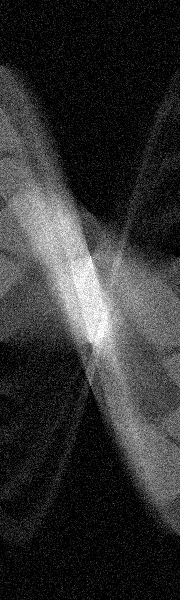
\includegraphics[height=5cm, width=3cm]{./figures/image-formation/sinogram_noisy.png}};
		\node at (0, -3) {\( p \)};
		\draw [-latex] (1.5, 0) -- ++(1, 0);
		\node [fill=photoncolor, draw=red!40!black, rectangle, minimum width=1cm, minimum height=1cm, thick] (den) at (3, 0) {\( \operatorname{den}_p \)};
		\draw [-latex] (3.5, 0) -- ++(1, 0);
		\node at (6, 0) {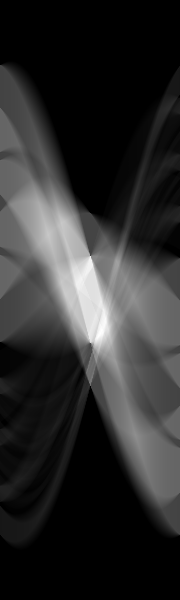
\includegraphics[height=5cm, width=3cm]{./figures/image-formation/sinogram.png}};
		\node at (6, -3) {\( p_\text{den} \)};
		\draw [-latex] (7.5, 0) -- ++(1, 0);
		\node [fill=secondary, draw=orange!40!black, draw, rectangle, minimum width=1cm, minimum height=1cm, thick] (rec) at (9, 0) {\( \operatorname{rec} \)};
		\draw [-latex] (9.5, 0) -- ++(1, 0);
		\node at (12, 0) {
\includegraphics[trim={0cm 5cm 0cm 5cm}, clip, width=3cm]{./figures/image-formation/fbpfull.png}};
		\node at (12, -2) {\( \hat{f} \)};

		\node [fill=photoncolor, draw=red!40!black, rectangle, text width=4cm, minimum height=1cm, thick] (denzoom) at (3, -2) {\small
				\ \textbullet\ Adaptive Filtering,\\
				\ \textbullet\ Total Variation,\\
				\ \textbullet\ feed-forward CNN, \ldots
		};
		\node [fill=secondary, draw=orange!40!black, rectangle, text width=2cm, minimum height=1cm, thick] (reczoom) at (9, -2) {\small
				\ \textbullet\ FBP,\\
				\ \textbullet\ SIRT,\\
				\ \textbullet\ ART, \ldots
		};
		\draw [thick, red!40!black] (den.south west) to [out=-100, in=10] (denzoom.north west);
		\draw [thick, red!40!black] (den.south east) to [out=-80, in=170] (denzoom.north east);
		\draw [thick, orange!40!black] (rec.south west) to [out=-100, in=30] (reczoom.north west);
		\draw [thick, orange!40!black] (rec.south east) to [out=-80, in=150] (reczoom.north east);
	\end{tikzpicture}
	\caption[Schematic of a pre-processing-based reconstruction pipeline.]{
		Schematic of a pre-processing-based reconstruction pipeline:
		The denoising algorithm \( \operatorname{den}_p \) yields the denoised sinogram (middle) from the noisy projections (left), which is subsequently used for reconstruction by any reconstruction algorithm \( \operatorname{rec} \) to finally yield the reconstructed image (right).
	}%
	\label{fig:learning:preprocessing scheme}
\end{figure}

Throughout the years, many approaches have been proposed, that approximately follow this scheme.
This ranges from the aforementioned pre-log Poisson denoising approaches over \gls{tv} and wavelet-based approaches~\cite{jiao_multiscale_2008,karimi_denoising_2016} to feed-forward \glspl{cnn}~\cite{ghani_cnn_2018}.
Although many of the characteristics of this approach are appealing, the reconstruction quality is typically lacking when compared to that of model-based iterative techniques.
Further, it is hard to have a profound intuition of the effect of \( \operatorname{den}_p \) on the final reconstruction.
\section{Post-processing}
The conceptual opposite of the Radon domain denoising is to perform denoising in the image domain, i.e.\ after reconstruction.
Here, we do not assume access to the projections \( p \), but only to the preliminary reconstruction \( \hat{f} \).
With this, we simply let
\begin{equation}
	\hat{f}_\text{den} = \operatorname{den}_{f}(\hat{f})
\end{equation}
be the final reconstruction, where \( \Func{\operatorname{den}_{f}}{\set{F}}{\set{F}} \) is an image-domain denoising algorithm.
As such, image-domain post-processing can easily extend any existing \gls{ct} workflow, without requiring access to any of the internals.
On the other hand, describing the noise in the image-domain is a very challenging task and usually inhibits deriving analytically optimal filtering strategies.
Many efforts have been made to adapt typical algorithms to this, e.g.\ \gls{nlm}~\cite{chen_thoracic_2012,li_adaptive_2013,ma_low_2011} and \gls{bm3d}~\cite{kang_image_2013}.

While these traditional methods are good at removing local incoherent noise, low-dose \gls{ct} typically exhibits coherent streaking artifacts.
Many learning-based approaches have been proposed to combat such artifacts~\cite{chen_low_2017,chen_low-dose_2017,liu_low-dose_2018,yang_improving_2017,zhao_convolutional_2019}.
Although the results are satisfactory, we emphasize that this discriminative learning setup expects to be applied to images with (at least) very similar corruptions --- that is, it assumes a particular forward model as well as reconstruction algorithm.
If this condition is not fulfilled, the preliminary reconstructions may exhibit artifacts that the \gls{cnn} can not remove.
\begin{figure}
	\centering
	\begin{tikzpicture}[scale=0.98]
		\node (noisy) at (0, 0) {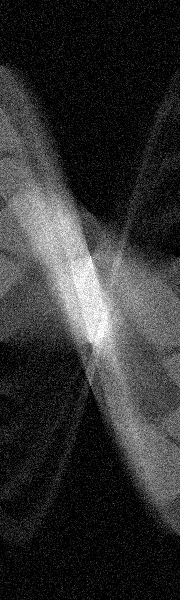
\includegraphics[height=5cm, width=3cm]{./figures/image-formation/sinogram_noisy.png}};
		\node at (0, -3) {\( p \)};
		\draw [-latex] (1.5, 0) -- ++(1, 0);
		\node [fill=secondary, draw=orange!40!black, rectangle, minimum width=1cm, minimum height=1cm, thick] (rec) at (3, 0) {\( \operatorname{rec} \)};
		\draw [-latex] (3.5, 0) -- ++(1, 0);
		\node at (6, 0) {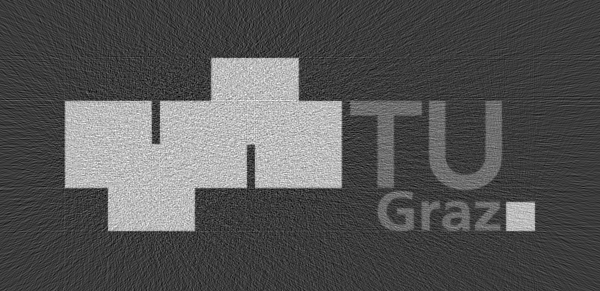
\includegraphics[width=3cm]{./figures/image-formation/noisy.png}};
		\node at (6, -1.3) {\( \hat{f} \)};
		\draw [-latex] (7.5, 0) -- ++(1, 0);
		\node [fill=photoncolor, draw=red!40!black, draw, rectangle, minimum width=1cm, minimum height=1cm, thick] (den) at (9, 0) {\( \operatorname{den}_f \)};
		\draw [-latex] (9.5, 0) -- ++(1, 0);
		\node at (12, 0) {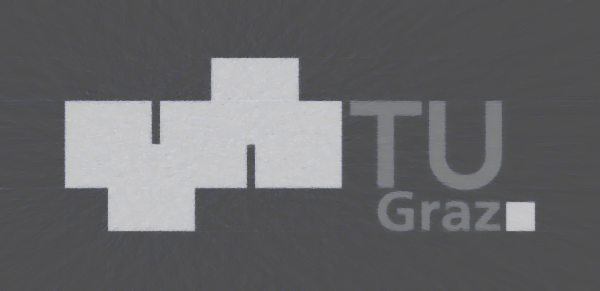
\includegraphics[width=3cm]{./figures/image-formation/rec_tv.png}};
		\node at (12, -1.3) {\( \hat{f}_\text{den} \)};

		\node [fill=photoncolor, draw=red!40!black, rectangle, text width=4cm, minimum height=1cm, thick] (denzoom) at (9, -2) {\small
				\ \textbullet\ Adaptive Filtering,\\
				\ \textbullet\ Total Variation,\\
				\ \textbullet\ feed-forward CNN, \ldots
		};
		\node [fill=secondary, draw=orange!40!black, rectangle, text width=2cm, minimum height=1cm, thick] (reczoom) at (3, -2) {\small
				\ \textbullet\ FBP,\\
				\ \textbullet\ SIRT,\\
				\ \textbullet\ ART, \ldots
		};
		\draw [thick, red!40!black] (den.south west) to [out=-100, in=10] (denzoom.north west);
		\draw [thick, red!40!black] (den.south east) to [out=-80, in=170] (denzoom.north east);
		\draw [thick, orange!40!black] (rec.south west) to [out=-100, in=30] (reczoom.north west);
		\draw [thick, orange!40!black] (rec.south east) to [out=-80, in=150] (reczoom.north east);
	\end{tikzpicture}
	\caption[Schematic of a post-processing-based reconstruction pipeline.]{
		Schematic of a post-processing-based reconstruction pipeline:
		The preliminary reconstruction \( \hat{f} \) is acquired by applying some standard reconstruction algorithm to the noisy sinogram \( p \), and subsequently denoised to yield the final reconstruction \( \hat{f}_\text{den} \).
	}%
	\label{fig:learning:postprocessing scheme}
\end{figure}
\section{Domain Transform Learning}
Another family of reconstruction techniques has emerged very recently with the increase of computational power.
Let us denote with \( (p, f) \in \set{P} \times \set{F} \) a pair of independent random variables with the associated joint distribution \( \distr{D} = \distr{p} \times \distr{f} \) on \( \set{P} \times \set{F} \).
An intriguing idea is to introduce an appropriately chosen parametric mapping \( \Func{r}{\set{P} \times \Phi}{\set{F}} \), such that
\begin{equation}
	\hat{f} = r(p, \optimal{\params}{}),%
	\label{eq:learning:automap mapping}
\end{equation}
where \( \optimal{\params}{} \in \Phi \subseteq \R^P \) is a parameter vector that is learned from data, for instance by minimizing the expected \( \ell_2 \) reconstruction error over \(\distr{D}\):
\begin{equation}
	\optimal{\params}{} = \argmin_{\params\in\Phi} \mathbb{E}_{(p, f) \sim \distr{D}} \Bigl[ \norm{r(p, \params) - f}_2^2 \Bigr].%
	\label{eq:learning:automap learning}
\end{equation}

Note that in this approach we do not require any domain knowledge at all.
That is, we do not require knowledge of the forward operator \( A \) or any other specifics of the acquisitions or reconstruction process.
We only require a dataset \( \set{D} \) that is distributed according to our specific measurement setup.
In this sense, this approach is very general and can as stated be applied to any reconstruction task.
In~\cite{zhu_image_2018}, the authors applied this framework to a range of medical imaging tasks, including \gls{ct} and \gls{mri} using different non-Cartesian sampling patters.

Although the results look promising, there are several problems with this approach.
As clearly indicated by~\cref{eq:learning:automap learning}, this approach is discriminative in nature.
As such, one is required to retrain \( r \) if the forward model changes, e.g.\ because a new undersampling pattern is discovered to be advantageous.
It also assumes access to both sensor-domain data and image-domain data, and assumes that there exists a known one-to-one association between them.
However, especially in the medical domain, data is in general sparse and one can not assume access to a high-quality dataset for every possible scanner geometry and sub-sampling strategy.
Further, due to the complete omission of the forward operator \( A \) in the reconstruction problem, it is clear that the parametric mapping \( r \) has to at least approximate it (more specifically, its \enquote{inverse}) somehow.
We want to emphasize that the forward models in medical imaging are usually \enquote{global} in some sense.
For instance, if we consider the \gls{fbp} example in~\cref{fig:image:simple backprojection example}, it is clear that changing one pixel in the sinogram affects the reconstruction along a line over its whole domain.
In \gls{mri}, where the sensor data is acquired in the Fourier domain, changes in the sensor domain change the reconstruction over its whole domain.
To account for this fact, the structure of \( r \) has to be chosen appropriately.
For instance, in the AUTOMAP framework~\cite{zhu_image_2018}, \( r \) is a neural network that utilizes fully connected layers in the early stages and convolutional layers in later stages.
The idea is to learn an approximate inverse of \( A \) in the early stages, and refine the reconstruction by changing the local structure in the later stages.
For larger resolutions, this poses a significant computational burden:
The number of parameters for one fully connected layer in an \gls{mri} reconstruction problem of resolution \( \num{512} \times \num{512} \) is \( \num{2} \times \num{512}^{\num{4}} = \num{137438953472} \), where the factor \( \num{2} \) arises from the complex data.
In general it can be concluded that, although appealing in some aspects, reconstruction by means of~\cref{eq:learning:automap mapping} is not feasible without restrictions on the resolution or specialized architecture considerations.
\section{Variational Reconstruction}
Previously, we outlined some approaches to reconstruction and highlighted some advantages as well as disadvantages.
In this section, we will discuss how we aim to solve the reconstruction problem throughout this thesis.
First, we will outline the framework of \emph{variational reconstruction}.
Then, we will specify our view on the problem and show how we aim to tackle it.
In a statistical framework, we will develop an image-domain prior on full \gls{ct}-images, such that we can enjoy all advantages of statistical modeling: Sampling from the prior as well as the posterior, computing different estimators, and rudimentary uncertainty quantification.

Let us again take a closer look at~\cref{eq:learning:forward}.
The system is usually overdetermined, since more projections are acquired, than there exist pixels in the reconstruction.
Further, the noise \( \nu \) prevents an exact solution in any case.
In general we can hope to reconstruct an image \( \optimal{f}{} \) that is consistent with the projections in the sense that it minimizes the re-projection error with respect to some metric \( \Func{d}{\set{P}\times\set{P}}{[0, \infty)}\). % chktex 9
For instance, for the least-squares estimator, we set \( d(Af, p) = \norm{Af - p}_2^2 \) and let
\begin{equation}
	\optimal{f}{LS} = \argmin_{f \in \set{F}} \norm{Af - p}_2^2.
\end{equation}
However, this is in general not satisfactory, as the solution will be guided by the noise \( \nu \) and the reconstruction will strongly depend on the specifics of the forward operator.
Therefore, we desire a way to incorporate prior knowledge into the solution, to guide it towards more \enquote{physically plausible} solutions.

In inverse problems, \emph{regularization} is the typical way to transform ill-posed problems into related well-posed problems.
A well-known regularization technique is due to Tikhonov~\cite{tikhonov_solution_1963}, who proposed to augment the least-squares objective by
\begin{equation}
	\optimal{f}{TK} = \argmin_{f \in \set{F}} \frac{1}{2}\norm{Af - p}_2^2 + \frac{\lambda}{2}\norm{f}_2^2%
	\label{eq:learning:tikhonov}
\end{equation}
which hinges on the assumption that \( \norm{f}_2^2 \) is \enquote{small} for plausible solutions.
Here, \( \lambda \in \R^+ \) is a parameter that controls the trade-off between \( f \) conforming to the measured data \( p \) and our prior assumption.
However, penalizing the magnitude of the reconstruction is rarely useful in imaging, as the solution would be biased towards low intensity images.

We can generalize~\cref{eq:learning:tikhonov} to the \emph{variational problem}
\begin{equation}
	\optimal{f}{} = \argmin_{f \in \set{F}}\ \bigl\{ E(f, p) \coloneq D(f, p) + R(f) \bigr\},%
	\label{eq:learning:variational}
\end{equation}
where the energy \( \Func{E}{\set{F} \times \set{P}}{\R} \) is composed of a \emph{data-fidelity term} \( \Func{D}{\set{F} \times \set{P}}{\R^+} \) which encodes the agreement of the reconstruction with the data, and a \emph{regularizer} \( \Func{R}{\set{F}}{\R} \) which penalizes solutions that are far from our prior assumptions on \( f \).
We immediately see that Tikhonov regularization sets \( D(f, p) = \frac{1}{2} \norm{Af - p}_2^2 \) and \( R(f) = \frac{\lambda}{2} \norm{f}_2^2 \).
\subsection{Statistical Interpretation}
In order to cast variational methods in the rigorous framework of statistical models, we first state that by Bayes rule, the posterior probability density \( \pdf{f \mid p}(\optimal{f}{}, p) \) of a reconstruction \( \optimal{f}{} \) given the data \( p \) is
\begin{equation}
	\pdf{f \mid p}(\optimal{f}{}, p) = \frac{\pdf{p \mid f}(\optimal{f}{}, p)\pdf{f}(\optimal{f}{})}{\int_{\set{F}} \pdf{p \mid f}(\params, p) \pdf{f}(\params)\ \dd \params},%
	\label{eq:learning:bayes}
\end{equation}
where \( \pdf{p \mid f} \) is the \emph{data likelihood} and \( \pdf{f} \) is the prior.
Similar to before, data likelihood describes the agreement between a solution \( \optimal{f}{} \) and the measured data \( p \).
Assuming an accurate characterization of \( \nu \), this is fully determined by the forward model~\cref{eq:learning:forward}.
On the other hand, the prior \( \pdf{f} \) should encode knowledge about the solution itself.
Note that the denominator of~\cref{eq:learning:bayes} is intractable for any realistic imaging task.
As an example, consider a discrete image of size \( \num{4} \times \num{4} \), where the pixel values are restricted to be in \(\{0,\dotsc,255\}\).
Then, \( |\set{F}| = \num{4294967296}\), which is already in a computationally prohibitive regime.
For an image of size \( \num{6} \times \num{6} \), \( |\set{F}| = \num{4.973232e+86} \) already surpasses most estimates of the number of baryons (e.g.\ protons and neutrons) in the observable universe.
Luckily, in most applications we do not require to calculate exact probabilities with \( \pdf{f \mid p} \), but we are mostly interested in finding maxima or sampling from it.

Assuming full knowledge of the (maybe unnormalized) posterior \( \pdf{f \mid p} \), we are typically interested in finding the solution which maximizes the posterior.
This is known as the popular \gls{map} estimator and reads
\begin{equation}
	\optimal{f}{MAP} = \argmax_{f \in \set{F}} \pdf{f \mid p}(f, p),%
	\label{eq:learning:map}
\end{equation}
which can be transformed into the negative-log domain as
\begin{equation}
	\optimal{f}{MAP} = \argmin_{f \in \set{F}} \big\{ -\log \pdf{p \mid f}(f, p) -\log\pdf{f}(f) \big\}.%
	\label{eq:learning:map neg log}
\end{equation}
If we interpret~\cref{eq:learning:variational} in this context, we see that the data-fidelity term \( D \) models the negative data log-likelihood \( -\log\pdf{p \mid f} \), while the regularizer \( R \) captures the negative log-prior \( -\log\pdf{f} \).

\subsection{Hand-crafted Regularizers}
While modeling the data-fidelity is usually straight forward, assuming the precise geometry of the scanner is known, finding a good regularizer for \gls{ct} images has been subject to years of research.
If we recall Tikhonov regularization, it is now clear that it is not well-suited for imaging applications, since it imposes a \enquote{small-magnitude} prior onto \( f \).
Therefore, it is interesting to consider other possible choices of \( R \).

A very fruitful idea is that of imposing a \enquote{smoothness} prior onto \( f \) by penalizing the image gradients.
One may initially be tempted to find
\begin{equation}
	\optimal{f}{Q} = \argmin_{f \in \set{F}} \frac{1}{2} \norm{Af - p}_2^2 + \frac{\lambda}{2} \norm{\mathrm{D} f}_F^2,
\end{equation}
where \( \Func{\mathrm{D}}{\R^N}{\R^{2 \times N}} \) is a discrete gradient operator and \( \norm{\cdot}_F \) is the Frobenius norm, which for a matrix \( B \in \R^{M \times N} \) is defined as \( \norm{B}_F = \sqrt{\sum_{m=1}^M \sum_{n=1}^N {(B_{m,n})}^2} \).
Since \( \frac{\lambda}{2} \norm{\mathrm{D} f}_F^2 \) models the negative log-prior, we can interpret this as assuming that the image gradients of \( f \) are normally distributed, with mean \num{0} and isotropic variance \( \frac{1}{\lambda} \).
However, this has the effect of smoothing edges in the image, which is generally not desirable.
To preserve sharp discontinuities in the image, a very popular approach is to penalize the \gls{tv}.
In this case, the regularizer is defined as
\begin{equation}
	R(f) = \lambda \norm{\mathrm{D} f}_{2, 1}
\end{equation}
where \( \norm{\cdot}_{2, 1} \) denotes the \( \ell_1  \) norm of the \( \ell_2 \) norm with respect to the columns.
That is,
\begin{equation}
	\norm{\mathrm{D} f}_{2, 1} = \sum_{n=1}^N \sqrt{{({(\mathrm{D} f)}_{1,n})}^2 + {({(\mathrm{D} f)}_{2,n})}^2}.
\end{equation}

The \gls{tv} regularizer and variations of it have been used extensively in the medical imaging domain as well as in problems concerning natural images.
For example, in~\cite{sidky_accurate_2006}, the authors apply the \gls{tv} regularizer to a limited-angle fan-beam reconstruction problem and extended this to a circular cone-beam setup in~\cite{sidky_reconstruction_2008}.
A well known drawback of the \gls{tv} regularizer is the staircasing effect~\cite{tang_performance_2009}, and many attempts have been made to overcome this~\cite{liu_total_2014,niu_sparse_2014,tian_reconstruction_2011,yang_high_2010,zhang_few-view_2013}.
As an example, we want to highlight the \gls{tgv}~\cite{bredies_total_2010}, which explicitly allows affine image profiles, and has been applied to a sparse-view reconstruction task~\cite{niu_sparse_2014}.
\subsection{Parametric Regularizers}
Although the \gls{tv} regularizer is very principled, it still left something to desire in terms of reconstruction quality.
The \gls{tgv} regularizer incorporated second-order statistics of the reconstruction and has been shown to improve quality of the reconstruction.
Therefore, it is convincing that considering higher-order statistics can improve reconstruction further.
However, modeling these statistics by hand becomes increasingly difficult, and it has been advocated quite early that proper modeling of (in this case natural) images should be based on \emph{learning} from data~\cite{zhu_filters_1998}.

In this work, we follow the approach of parametrizing our regularizer such that~\cref{eq:learning:variational} changes to
\begin{equation}
	\optimal{f}{} = \argmin_{f \in \set{F}}\ \bigl\{ E(f, p, \params) \coloneq D(f, p) + R(f, \params) \bigr\},%
	\label{eq:learning:parametrized inference}
\end{equation}
where \( \params \in \Phi \subset \R^P \) are the parameters that should be learned from data.
Now, the energy \( \Func{E}{\set{F} \times \set{P} \times \Phi}{\R} \) measures the compatibility between a reconstruction \( f \in \set{F} \) and the data \( p \in \set{P} \) given the learned parameters \( \params \).
In our approach, the data fidelity term remains unchanged, but we parametrize the regularizer \( \Func{R}{\set{F} \times \Phi}{\R} \) which encodes prior knowledge on \( f \) using the learned parameters \( \params \).

Although typically not used in the medical imaging domain, we want to highlight the prolific \gls{foe} regularizer due to Roth and Black~\cite{roth_fields_2005}.
For an image \( f \in \R^N \), the \gls{foe} regularizer is defined as
\begin{equation}
R_{\text{FoE}}(f, \params) = \sum_{n=1}^N \sum_{j=1}^J \psi({(K_j f)}_n, w_j)
\end{equation}
where the parameters are summarized as \( \params = {(k_j, w_j)}_{j=1}^J \), with \( k_j \in \R^{a^2} \) a convolution filter of size \( a \times a \) corresponding to the linear operators \( K_j \in \R^{N \times N} \).
In more detail, the potential functions \( \Func{\psi}{\R \times \R^{N_w}}{\R} \) are parametrized by the weights \( w_j \in \R^{N_w} \), where a typical choice of parametrization may be to use radial basis functions
\begin{equation}
	\psi(x, w) = \sum_{k=1}^{N_w} w_k \exp\Bigl( -\frac{x - \mu_k}{\sigma} \Bigr).
\end{equation}
Here, \( \mu_k \) are equidistantly spaced within some interval and \( \sigma \) is chosen a-priori to capture the range of the filter responses.
Clearly, the receptive field of the \gls{foe} regularizer is determined by the filter size \( a \).
This is a drawback for medical imaging applications, where artifacts typically appear as coherent streaks over a large footprint.

In this section, we have demonstrated the idea of parametric regularizers and gave as an example the well known \gls{foe} model.
Before we can apply any parametric regularizer to an inference task such as~\cref{eq:learning:parametrized inference}, we have to first identify the parameters such that the regularizer encodes useful prior information.
In the next sections, we will discuss how we can learn the parameters for a regularizer in an energy of the form~\cref{eq:learning:parametrized inference}.
\section{Parameter Identification}
Typical regularizers that are used today in the field of medical imaging or natural image restoration have hundreds, thousands, or hundreds-of-thousands parameters.
Clearly, is is not feasible to tune these parameters by hand, and we therefore require ways to learn these parameters from data.
In this section, we want to explore ways of learning the parameters of a regularizer for an energy of the form of~\cref{eq:learning:parametrized inference}.

First, we want to highlight that in our energy formulation, we only parametrize the regularizer \( R \).
\( R \) encodes prior information on \( f \), and is independent of any measurements \( p \).
As such, one may be tempted to think that we can not incorporate some known one-to-one mappings between \( p \) and \( f \) for learning \( \params \).
However, there do exist ways to learn the posterior in a supervised~\cite{bishop_pattern_2006,murphy_machine_2012} manner, and we want to discuss these first, although this is not the approach that we follow in this thesis.
\subsection{Bilevel Optimization}
By means of bilevel optimization, we can learn the parameters of a regularizer in a supervised manner~\cite{kunisch_bilevel_2013}, whereby we solve a higher- and lower-level optimization problem.
To be more precise, let \( (f_\text{GT}, \nu) \in \set{F} \times \R^M \) denote a pair of independent random variables distributed according to \( \distr{D} = \distr{f} \times \distr{\nu} \).
The bilevel optimization approach is to minimize the reconstruction error, where the reconstruction is the minimizer of a lower-level optimization problem, that is
\begin{equation}
	\begin{cases}
		\displaystyle \optimal{\params}{BO} = \argmin_{\params \in \Phi} \mathbb{E}_{(f_\text{GT}, \nu) \sim \distr{D}} \bigl[ \mathcal{L}(\optimal{f}{}(f_\text{GT}, \nu), f_\text{GT}) \bigr], \\
		\displaystyle \st\ \optimal{f}{}(f_\text{GT}, \nu) = \argmin_{f \in \set{F}} \frac{1}{2} \norm{Af - p}_2^2 + R(f, \params).
	\end{cases}
\end{equation}
Here, \( \Func{\mathcal{L}}{\set{F} \times \set{F}}{\R^+} \) is a continuously differentiable loss function and we require \( R \) to be twice continuously differentiable.
The problem can be solved using Lagrange multiplier theory and implicit differentiation~\cite{samuel_learning_2009}.
Note that the lower-level problem typically has to be solved with high precision, which can be computationally expensive.
\subsection{Truncated Optimization}
A significant drawback of bilevel optimization approaches is the computational burden associated with solving the lower level problem.
The idea behind truncated optimization~\cite{barbu_training_2009,domke_generic_2012} is to replace the minimization with an approximate scheme, e.g.\ fixed-step gradient descent.
That is, we aim to solve
\begin{equation}
	\begin{cases}
		\displaystyle \optimal{\params}{TO} = \argmin_{\params \in \Phi} \mathbb{E}_{(f_\text{GT}, \nu) \sim \distr{D}} \bigl[ \mathcal{L}(\optimal{f}{T}(f_\text{GT}, \nu), f_\text{GT}) \bigr], \\
		\displaystyle \st\ \optimal{f}{t+1}(f_\text{GT}, \nu) = \optimal{f}{t}(f_\text{GT}, \nu) -\tau \bigl(A^*(A\optimal{f}{t}(f_\text{GT}, \nu) - p) + \nabla_1 R(\optimal{f}{t}(f_\text{GT}, \nu), \params)\bigr).
	\end{cases}%
	\label{eq:learning:truncated optimization}
\end{equation}
for \( \text{t} = 0, \dotsc, \text{T} - 1 \) given some initial estimate \( \optimal{f}{0} \), where \( A^* \) denotes the adjoint of \( A \), \( \nabla_N \) is the gradient w.r.t.\ the \(N\)-th argument, and \( \tau \) is an appropriately chosen step size.
We see that in this fixed-step gradient descent scheme, we can directly propagate the gradient of the loss function through the iterative procedure.
It can be shown that under certain conditions, the gradients w.r.t.\ the parameters of the bilevel problem and the truncated problem converge~\cite{mehmood_automatic_2020}.

At this point, we want to quickly note that while both the bilevel and truncated approach learn the posterior, they can still be interpreted in the framework of energy-based models.
An interesting idea is to abandon this framework, and parametrize each of the descent steps in~\cref{eq:learning:truncated optimization} individually.
We point the interested reader to~\cite{chen_learn_2018}, where the authors applied this idea to a sparse-view \gls{ct} reconstruction problem.
\subsection{Maximum Likelihood Learning}
The strategies that we discussed in the previous sections aim to, in some sense, learn the posterior distribution directly.
While this has some benefits (mainly better discriminative performance), it also has drawbacks:
We again assume that we have access to data-image pairs, and the posterior that we learn is tailored to a specific reconstruction problem.
In this section, we want to detail a fully generative approach, which does not assume access to measurements at all, and is independent of any particular acquisition setup.
We will use this approach to train a full-image regularizer that operates on multiple scales.
We detail the specifics of our setup in~\cref{sec:experiments}.

A very well known statistical parameter fitting framework is that of \gls{ml}, where we aim to fit our model to the data, such that the likelihood of the data under our model is maximized.
Specifically, we interpret \gls{ct} images \( f \in \set{F} \subseteq \R^N \) of size \( N = N_v \times N_h \) as random variables distributed according to \( \distr{f} \).
To associate a distribution with our regularizer, we follow the maximum-entropy principle~\cite{zhu_filters_1998}, such that the probability density reads as
\begin{equation}
	\pdf{M}(f, \theta) = \frac{\exp(-R(f, \params))}{\int_{\set{F}} \exp(-R(\zeta, \params))\ \dd \zeta}.%
	\label{eq:learning:model density}
\end{equation}
\( \pdf{M} \) is often called the \emph{Gibbs-Boltzmann} density of \( R \), and we denote the induced distribution by \( \distr{M} \).

To find the maximum likelihood estimate \( \optimal{\params}{ML} \in \Phi \), we can equivalently minimize the expected negative-log likelihood \( \mathbb{E}_{f \sim \distr{f}} [-\log \pdf{M}(f, \params)]\), which amounts to
\begin{equation}
	\optimal{\params}{ML} = \argmin_{\params \in \Phi}\ \Biggl\{\, \NLL(\params) \coloneq \mathbb{E}_{f \sim \distr{f}}[R(f, \params)] + \log\biggl( \int_{\set{F}} \exp(-R(\zeta, \params))\ \dd\zeta \biggr)\,\Biggr\}.
\end{equation}
The gradient of the \gls{ml} objective with respect to \( \params \) is found to be
\begin{equation}
	\grad{1} \NLL(\params) = \mathbb{E}_{f \sim \distr{f}} [\grad{2} R(f, \params)] - \int_{\set{F}} \underbrace{\frac{\exp(-R(\zeta, \params))}{\int_{\set{F}} \exp(-R(\hat{\zeta}, \params))\ \dd \hat{\zeta}}}_{\pdf{M}(\zeta, \params)} \grad{2} R(\zeta, \params)\ \dd \zeta,
\end{equation}
where we identify the second term to be the expected gradient under the model distribution, such that we arrive at
\begin{equation}
	\grad{1} \NLL(\params) = \mathbb{E}_{f^+ \sim \distr{f}} \bigl[ \grad{2}R(f^+, \params) \bigr] - \mathbb{E}_{f^- \sim \distr{M}} \bigl[ \grad{2} R(f^-, \params) \bigr].%
	\label{eq:learning:ml objective final}
\end{equation}
Thus, the gradient of the maximum likelihood objective is the difference between the expected gradient of \gls{ct} images and the expected gradient of samples from the model distribution.
Therefore, training with~\cref{eq:learning:ml objective final} has the effect of decreasing the regularization cost of samples from the data distribution, while increasing the regularization cost of \enquote{hallucinations} produced by the model.
We want to quickly note that this objective also arises in Kullback-Leibler divergence minimization, where the Kullback-Leibler divergence reads
\begin{equation}
	(\distr{f} || \distr{M}) = \int_{\set{F}} \pdf{f}(\zeta) \log \frac{\pdf{f}(\zeta)}{\pdf{M}(\zeta, \params)}\ \dd \zeta = -\operatorname{H}(\distr{f}) - \mathbb{E}_{f \sim \distr{f}} [\log \pdf{M}(f, \params)].
\end{equation}
With the entropy \( \operatorname{H} \) of \( \distr{f} \) independent of \( \params \), we conclude that
\begin{equation}
	\argmin_{\params \in \Phi}\ (\distr{f} || \distr{M}) = \argmin_{\params \in \Phi} \NLL(\params).
\end{equation}

We want to emphasize that this method of parameter identification only relies on \( \distr{f} \).
That is, we do not require any measurement data during learning, and our model does not depend on any specific forward operator \( A \) or noise distribution \( \distr{\nu} \).
Since we learn an independent prior (as opposed to the posterior learning from the previous approaches), we also gain the ability to sample our model, such that we can gain valuable insight into what was learned.
This comes at the price of an increased computational cost of sampling \( \distr{M} \), where one typically has to resort to computationally expensive \gls{mcmc} methods.
We will discuss different samplers that could be used in the imaging domain in the next section.

It has been pointed out by Hinton~\cite{hinton_training_2002} that estimating the expected gradient with respect to the induced model distribution \( \distr{M} \) is computationally very challenging and often leads to high-variance estimates.
Therefore, he proposed to change~\cref{eq:learning:ml objective final} to
\begin{equation}
	\grad{1} \NLL(\params) \approx \mathbb{E}_{f^+ \sim \distr{f}} \bigl[ \grad{2}R(f^+, \params) \bigr] - \mathbb{E}_{f^- \sim \distr{M^T}} \bigl[ \grad{2} R(f^-, \params) \bigr],%
	\label{eq:learning:contrastive divergence}
\end{equation}
where \( \distr{M^T} \) is the induced model distribution after applying some \gls{mcmc} transition operator (e.g.\ Gibbs sampling~\cite{geman_stochastic_1984}) to \( \distr{f} \), \( T \in \mathbb{N}^+ \) times.
This approximation, known as the \gls{cd} objective, removes almost all of the computational complexity associated with sampling the model if \( T \) is small, and yet yields a reasonable, although biased~\cite{perpinan_contrastive_2005}, approximation of the gradient.

\gls{cd}-based training has historically been used extensively in image restoration problems, with the influential \gls{poe}~\cite{hinton_training_2002} and \gls{foe}~\cite{roth_fields_2005} models both being trained in this framework.
Subsequently, these approaches have fallen out of favor for improved discriminative performance, for instance by using~\cref{eq:learning:truncated optimization}.
However, recently the \gls{ml} framework has received increasing attention, especially for its generative capabilities~\cite{du_implicit_2019,nijkamp_shortrun_2019}.
New models can rival the generative performance of \glspl{gan}~\cite{goodfellow_generative_2014}, while preserving the strengths of the probabilistic framework, such as composability, interpretability, and stability due to the lack of an explicit generator network~\cite{du_improved_2020,nijkamp_anatomy_2019}.

In this work, we want to build up on the generative capabilities of this approach.
That is, we aim to construct a multi-scale network which we train with~\cref{eq:learning:contrastive divergence}, such that we can sample full-sized images from our model.
This is in contrast to, e.g., the \gls{foe} regularizer, which, although also traditionally trained with~\cref{eq:learning:contrastive divergence}, can only encode local information.
\subsubsection{Model Sampling}
In the previous section, we derived the objective for fitting a parametric regularizer to data, such that its maximum-entropy distribution maximized the likelihood of the data.
The gradient of this loss function with respect to the parameters \( \params \) of the model, as seen in~\cref{eq:learning:ml objective final}, is composed of two terms:
The expected gradient with respect to samples \( f^+ \) drawn from the data distribution \( \distr{f} \), and the negative expected gradient with respect to samples \( f^- \) drawn from the induced model distribution \( \distr{M} \).
While the first term is easily approximated given a data set drawn from \( \distr{f} \), the second term requires sampling from the model, which is achieved by using \gls{mcmc} methods.

There are many approaches to sample from an unnormalized density~\cite[Chapter~11]{brooks_handbook_2011,bishop_pattern_2006}, which include Gibbs sampling~\cite{geman_stochastic_1984}, Metropolis-Hastings sampling~\cite{hastings_monte_1970}, Hybrid Monte Carlo~\cite{douane_hybrid_1987}, and \gls{lmc}~\cite{roberts_optimal_1998}.
In this work we restrict ourselves to samplers that
\begin{enumerate*}
	\item make use of the local landscape of the density, and
	\item simultaneously update all entries in the underlying random vector.
\end{enumerate*}
The reasons for this are of practical nature:
Samplers that update entries sequentially, such as Gibbs sampling, are impractical for any reasonably sized image (e.g.\ \( \num{512} \times \num{512} = \num{262144} \) entries) in terms of computation.
Similarly, using the local landscape (i.e.\ the gradient) of the density allows for faster convergence of the Markov chains.

We now detail the sampling strategy used in this thesis, which is \gls{lmc}~\cite{grenader_representations_1994,nijkamp_shortrun_2019,roberts_exponential_1996,rossky_brownian_1978}.
\gls{lmc} makes use of the gradient of the underlying density during sampling, which improves mixing time when compared to, e.g.\ Gibbs sampling.
Recall that our objective is to sample from \( \distr{M} \), whose associated density is given by~\cref{eq:learning:model density}, which we repeat as
\begin{equation}
	\pdf{M}(f, \params) = \frac{\exp(-R(f, \params))}{\int_{\set{F}} \exp(-R(\zeta, \params))\ \dd \zeta}.\nonumber
\end{equation}
In the general class of Metropolis-Hastings algorithms, there exists a proposal distribution with associated density \( \pdf{P}(f, f^{\rightarrow}) \) on \( \set{F} \times \set{F} \).
A candidate \( f^{\rightarrow} \) is drawn from the proposal distribution and the transition is accepted with probability
\begin{equation}
	\alpha(f, f^{\rightarrow}) = \begin{cases}
		\min\left\{ \frac{\pdf{M}(f^{\rightarrow}, \params)\pdf{P}(f^\rightarrow, f)}{\pdf{M}(f, \params)\pdf{P}(f, f^\rightarrow)}, 1\right\}, &\ \text{if}\ \pdf{M}(f, \params) \pdf{P}(f, f^{\rightarrow}) > 0, \\
		1, &\ \text{if}\ \pdf{M}(f, \params) \pdf{P}(f, f^{\rightarrow}) = 0.
	\end{cases}%
	\label{eq:learning:metropolis hastings step}
\end{equation}
This choice of \( \alpha \) can be shown to be \( \pdf{M} \)-invariant, in the sense that
\begin{equation}
	\pdf{M}(f, \params) = \int_{\set{F}} \pdf{M}(\xi, \params) \pdf{P}(\xi, f) \alpha(\xi, f)\ \dd \xi
\end{equation}
and that the transition probabilities converge to \( \pdf{M} \).
The proposal density we consider is derived from Langevin diffusion:
Let \( f^{t - 1} \) be the current state of the chain, then the proposal distribution takes the form
\begin{equation}
	f^t \sim \mathcal{N}(f^{t - 1} + \frac{\epsilon}{2}\grad{1} \log \pdf{M}(f^{t - 1}, \params), \epsilon\Id{N}),%
	\label{eq:learning:langevin proposal}
\end{equation}
where \( \mathcal{N}(\mu, \Sigma) \) denotes the normal distribution on \( \R^N \) with mean \( \mu \) and covariance matrix \( \Sigma \).

\gls{lmc} is also known as the \gls{mala} due to the Metropolis-Hastings step~\cref{eq:learning:metropolis hastings step}.
In practice, the Metropolis-Hastings acceptance step is often simply omitted~\cite{du_implicit_2019,nijkamp_anatomy_2019}, leading to the \gls{ula} which only approximately maintains \( \pdf{M} \) as the invariant distribution.
This can be illustrated by the following example taken from~\cite{roberts_exponential_1996}:
Assume that \( \distr{M} = \mathcal{N}(0, 1) \) on \( \R \) and \( \epsilon = 2 \), from which it immediately follows that \( f^t \sim \mathcal{N}(0, 2) \), \( t \in \mathbb{N}^+ \).
That is, the chain immediately converges, but samples are not distributed according to \( \distr{M} \).
We summarize \gls{mala} and the unadjusted variant in~\cref{alg:learning:mala}.
\begin{algorithm}[t]
	\DontPrintSemicolon
	\SetKwInOut{Input}{Input}
	\SetKwInOut{Output}{Output}
	\Input{Initial point \(f^0\), step size \(\epsilon\), Langevin steps \( T \)}
	\Output{\( f^T \)}
	\For{\( t = 1,\dotsc,T\)}{
		Propose \( f^\rightarrow \) with~\cref{eq:learning:langevin proposal}.\;
		Compute \( \alpha(f^{t-1}, f^\rightarrow) \) by \(
			\begin{cases}
				\cref{eq:learning:metropolis hastings step} &\ \text{for \gls{mala}},\\
				\alpha(f^{t-1}, f^\rightarrow) = 1 &\ \text{for \gls{ula}}.
			\end{cases}
		\)\;
		Draw \( r \sim \mathcal{U}[0, 1] \).\;
		Set \( f^t = \begin{cases}
			f^\rightarrow &\ \text{if}\ r < \alpha,\\
		f^{t - 1} &\ \text{else}.\end{cases} \)\;
	}
	\caption{\gls{mala} and \gls{ula} for sampling from an (unnormalized) density.}%
	\label{alg:learning:mala}
\end{algorithm}
\end{document}
